\begin{figure}[t]
    \centering
    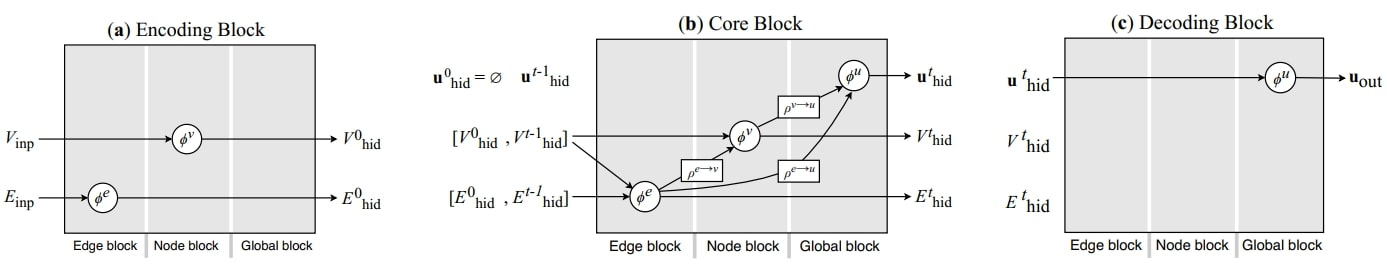
\includegraphics[width=1.0\textwidth]{figures/images/ch4/computational_flow.jpg}
    \caption{Computational flow of the STRIPS-HGN model \cite{shen2020learning}, consisting of three main blocks: Encoding, Core, and Decoding. The Encoding Block generates initial hidden representations for both node and edge embeddings. The Core Block implements the message-passing mechanism, updating the hidden representations of nodes, edges, and global embeddings. Finally, the Decoding Block generates the output graph, where the global embedding represents the predicted heuristic value.}
    \label{fig:computation_flow}
\end{figure}
